\documentclass[12pt]{article}
\usepackage{listings}
\usepackage{color}
\usepackage{enumitem}
\usepackage{amsmath}
\usepackage{hyperref}
\usepackage{pgfplots}
\usepackage{circuitikz}
\usetikzlibrary{positioning}

\definecolor{dkgreen}{rgb}{0,0.6,0}
\definecolor{gray}{rgb}{0.5,0.5,0.5}
\definecolor{mauve}{rgb}{0.58,0,0.82}

\lstset{frame=tb,
  language=Bash,
  aboveskip=3mm,
  belowskip=3mm,
  showstringspaces=false,
  columns=flexible,
  basicstyle={\small\ttfamily},
  breaklines=true,
  breakatwhitespace=true,
  tabsize=3
}

\author{Michał Tracewicz}
\date{2020-03-07}
\title{\LaTeX - Introduction}
\begin{document}
\pagenumbering{gobble}
\maketitle
\newpage
\tableofcontents
\newpage
\pagenumbering{arabic}
\section{What is \LaTeX?}
\LaTeX is a markup language to typeset documents.
It can be understood as a way to programaticly create documents.
\section{Compiling document}
Document writen using \LaTeX need to be compiled before they are rendered into output file.
First of user needs to install \LaTeX. In Ubuntu Linux this can be done with following commands:
\begin{lstlisting}
    sudo apt install textlive
    sudo apt-get install texlive-latex-extra
\end{lstlisting}
User should create '.tex' file in which they write their document using \LaTeX.
Afterwards this document should be compiled using following command:
\begin{lstlisting}
    pdflatex [source file path]
\end{lstlisting}
It will produce '.pdf' file in current directory.
\section{Document structure}
\subsection{Basic document structure}
\LaTeX uses commands to do format, structureing document etc.
For exaple:
\begin{verbatim}
    \section{Name}
\end{verbatim}
This will create numbered section in document with heading "Name".
Basic \LaTeX document should look something like this:
\begin{verbatim}
\documentclass{article}
\begin{document}
  Hello World!
\end{document}
\end{verbatim}
It begins with with:
\begin{verbatim}
\documentclass{article}
\end{verbatim}
All of \LaTeX comands starts with '\textbackslash'.
First line of our document should be documentclass command.
It determins how the whole document will be rendered. "article" is one of most common classes. Other notable
options are "book", "report", "slides", "beamer" (the last one is used to create presentations).
Next we have:
\begin{verbatim}
\begin{document}
    Hello World!
\end{document}
\end{verbatim}
Here we create an environment. It is possible to create multiple environments in one document.
They are parts of document to which certain typeseting rules applay.
Inside it author inserts content of theirs document.
Everything which will be put between those two segments is called a "Preamble".
Here user can point which packages will be used (more on this later), insert metadata from which
document title page will be created. Things which are in preamble will not be directly rendered on document.
For exaple lets take a look at part of this documents preamble:
\begin{verbatim}
\documentclass[12pt]{article}
\usepackage{listings}

\author{Michał Tracewicz}
\date{2020-03-07}
\title{\LaTeX - Introduction}

\begin{document}
\pagenumbering{gobble}
\maketitle
\newpage
\pagenumbering{arabic}
\end{document}
\end{verbatim}
Document title, author and date are inserted and then later on rendered with:
\begin{verbatim}
    \maketitle
\end{verbatim}
Looking at this snippet there are some more interesting commands
\begin{verbatim}
    \pagenumbering{gobble}
    \newpage
    \pagenumbering{arabic}
\end{verbatim}
Going top to bottom first user disables title page from being numbered. Then user forces new page to make sure 
only title is placed on first page. Next command enables numbering of pages using arabic numbers.
To force \LaTeX to create new line use "\textbackslash\textbackslash",
to force new line use "\textbackslash newline", new page "\textbackslash newpage"
\subsection{Sections, paragraphs}
\LaTeX gives its users a way to automaticly create and number section headings.
In addition user can create headings without numbering using paragraphs.
To structure document one can use those commands:
\begin{verbatim}
    \section{Section name}
    \subsection{Subsection name}
    \subsubsection{Subsubsection name}

    \paragraph{Paragraph name}
    \subparagraph{Subparagraph name}
\end{verbatim}
\subsection{Packages}
\LaTeX has a lot of both user created and built in packges.
To find packages visit: \href{https://www.ctan.org/pkg}{ctan.org}
User can download and remove packages by using:
\begin{lstlisting}
tlmgr install <package1> <package2> ...
tlmgr remove <package1> <package2> ...
\end{lstlisting}
To use package we need to register it using
\begin{verbatim}
\usepackage{listings}
\end{verbatim}
Doing so will give user ability to use commands provided in package.
This particular package provides way to do source code highlighting.
It will be described in later section.
\subsection{Table of contents}
If user had used sections to structure theirs document \LaTeX provides a command to create table of contents
based secotions, subsections,subsubsections.
\begin{verbatim}
    \tableofcontents
\end{verbatim}
\subsection{Lists}
When writing \LaTeX documents user has an ability to create both ordered and unordered lists.
\subsubsection{Unordered lists}
Following snippet can be used to create unordered list which will contain three entries named
"First", "Second", "Third":
\begin{verbatim}
    \begin{itemize}
        \item First
        \item Second
        \item Third
    \end{itemize}
\end{verbatim}
This wil render as:
\begin{itemize}
    \item First
    \item Second
    \item Third
\end{itemize}
When working with unordered lists sometimes it is desierable to change item symbol.
This can be done by:
\begin{verbatim}
    \begin{itemize}
        \item[--] Dash
        \item[$\ast$] Asterisk
        \item[$\beta$] Any mathematical symbol
    \end{itemize}
\end{verbatim}
Which will render as:
\begin{itemize}
    \item[--] Dash
    \item[$\ast$] Asterisk
    \item[$\beta$] Any mathematical symbol
\end{itemize}
To change symbol for all elements we will use package and it will be 
demonstrated in Ordered List section.
\subsubsection{Ordered lists}
Following snippet can be used to create ordered list which will contain three entries named
"First", "Second", "Third":
\begin{verbatim}
    \begin{enumerate}
        \item First
        \item Second
        \item Third
    \end{enumerate}
\end{verbatim}
This will render as:
\begin{enumerate}
    \item First
    \item Second
    \item Third
\end{enumerate}
Changeing enumeration can be done in two steps.
First user needs to add this to theirs preamble:
\begin{verbatim}
    \usepackage{enumitem}
\end{verbatim}
Then we can use following:
\begin{verbatim}
% Roman numbers
\begin{enumerate}[label=(\roman*)]
    \item First
    \item Second
    \item Third
\end{enumerate}

% Arabic numbers
\begin{enumerate}[label=\arabic*)]
    \item First
    \item Second
    \item Third
\end{enumerate}

% Alphabetical
\begin{enumerate}[label=\alph*)]
    \item First
    \item Second
    \item Third
\end{enumerate}
\end{verbatim}
Which will render as:
\begin{enumerate}[label=(\roman*)]
    \item First
    \item Second
    \item Third
\end{enumerate}
\begin{enumerate}[label=\arabic*)]
    \item First
    \item Second
    \item Third
\end{enumerate}
\begin{enumerate}[label=\alph*)]
    \item First
    \item Second
    \item Third
\end{enumerate}
This can also be used to change symbols in unordered lists:
\begin{verbatim}
    \begin{itemize}[label=$\ast$)]
        \item First
        \item Second
        \item Third
    \end{itemize}
\end{verbatim}
Which will render as:
\begin{itemize}[label=$\ast$)]
    \item First
    \item Second
    \item Third
\end{itemize}
\subsubsection{Nested lists}
Following snippet can be used to create nested ordered list which will contain five entries named
"First" - it will contain subentries "Second" and "Third", "Fourth", "Fifth"
\begin{verbatim}
    \begin{enumerate}
        \item First
        \begin{enumerate}
            \item Second
            \item Third
        \end{enumerate}
        \item Fourth
        \item Fifth
    \end{enumerate}
\end{verbatim}
This will render as:
\begin{enumerate}
    \item First
    \begin{enumerate}
        \item Second
        \item Third
    \end{enumerate}
    \item Fourth
    \item Fifth
\end{enumerate}
\subsection{Footnotes}
In \LaTeX there are is an easy way of creating and refering footnotes.
\begin{verbatim}
    Example \footnote{\label{myfootnote} Hello footnote}
    Refering to footnote \ref{myfootnote}
\end{verbatim}
Which will render as:
Example \footnote{\label{myfootnote} Hello footnote}
Refering to footnote\ref{myfootnote}
Footnotes are numbered automaticly.
It is imperative, that the label is contained in footnote,
otherwise the label will refer to section
\section{Mathematics}
\LaTeX is designed in a way which makes it easy to insert mathematical equations.
There are two options how user can handle inputing maths into document.
The first one is embeding the formula inline directly into the text.
This can be done using \$.
For example:
\begin{verbatim}
    Exponential functions can look like this: $f(x) = 2^x$
\end{verbatim}
Which will render as:
Exponential functions can look like this: $f(x) = 2^x$
Second option includes creating new environment.
Two main math environments are "equation" which is used to render one equation 
(if user trys to enter more it will resault in compilation error)
and "align" which is used to render multiple equations at the same time.
Examples:
\begin{verbatim}
    \usepackage{amsmath}
    % Code omitted for clarity...
    \begin{equation*}
        f(x) = \frac{1}{x}
    \end{equation*}
    \begin{align*}
        1 + 2x &= 3 \\
            3x &= 5 - 2
    \end{align*}
\end{verbatim}
This will be renddered as:
\begin{equation*}
    f(x) = \frac{1}{x}
\end{equation*}
\begin{align*}
    1 + 2x &= 3 \\
        3x &= 5 - 2
\end{align*}
Lets take a closer look at "align" environment.
As its name sugests, it will align equations. This will happen at '\&' sign.
Each equation needs to be separeted with "\textbackslash\textbackslash".
Asterisk at the end of both environments are used to indicate that user doesn't want them to be numbered.
\LaTeX is capable of displaying much more complicated equations some notable examples:
\begin{verbatim}
\begin{align*}
\left[
\begin{matrix}
1 & 0\\
0 & 1
\end{matrix}
\right]
&\ast
\left[
\begin{matrix}
a & b\\
c & d
\end{matrix}
\right]
=
\left[
\begin{matrix}
a & b\\
c & d
\end{matrix}
\right]\\
&\int^b_a\left(\frac{1}{\sqrt{x\pi}}\right)\\
T^{i_1 i_2 \dots i_p}_{j_1 j_2 \dots j_q} &= T(x^{i_1},\dots,x^{i_p},e_{j_1},\dots,e_{j_q})
\end{align*}
\end{verbatim}
Which is rendered as:
\begin{align*}
\left[
\begin{matrix}
1 & 0\\
0 & 1
\end{matrix}
\right]
&\ast
\left[
\begin{matrix}
a & b\\
c & d
\end{matrix}
\right]
=
\left[
\begin{matrix}
a & b\\
c & d
\end{matrix}
\right]\\
&\int^b_a\left(\frac{1}{\sqrt{x\pi}}\right)\\
T^{i_1 i_2 \dots i_p}_{j_1 j_2 \dots j_q} &= T(x^{i_1},\dots,x^{i_p},e_{j_1},\dots,e_{j_q})\\
\lim^{}_{x->\inf}\frac{1}{x} &= 0
\end{align*}
Lets take a closer look. To create matrix user creates
\begin{verbatim}
\left[
\begin{matrix}
a & b\\
c & d
\end{matrix}
\right]
\end{verbatim}
\textbackslash left[ and \textbackslash right] are responsible for creatinon of scaling braces around matrix.
Then it is created using "matrix" environment, 
new line character ("\textbackslash\textbackslash") is responsible for creating new row.
\textbackslash int - integral symbol\\
\textbackslash frac - fractions\\
\textbackslash sqrt - squere root\\
"\textasciicircum\{a\}\_\{b\}" - is used to create indexes where "a" is top and "b" is bottom)\\
\textbackslash dots - inserts "..."\\
\textbackslash pi - inserts Pi symbol (any greek letter can be inserted in the same fashion)\\
\section{Pictures}
\section{Bibliography}
\section{Tables}
To create tables user needs to combine two environments, "table" and "tabular".
Example code to create table looks like this:\\
\begin{verbatim}
\begin{table}[h!]
\begin{center}
    \caption{Your first table.}
    \label{tab:table1}
    \begin{tabular}{l|c|r}
    \textbf{Value 1} & \textbf{Value 2} & \textbf{Value 3}\\
    $\alpha$ & $\beta$ & $\gamma$ \\
    \hline
    1 & 1110.1 & a\\
    2 & 10.1 & b\\
    3 & 23.113231 & c\\
    \end{tabular}
\end{center}
\end{table}
\end{verbatim}
Which will render as:
\begin{table}[h!]
\begin{center}
    \caption{Your first table.}
    \label{tab:table1}
    \begin{tabular}{l|c|r}
    \textbf{Value 1} & \textbf{Value 2} & \textbf{Value 3}\\
    $\alpha$ & $\beta$ & $\gamma$ \\
    \hline
    1 & 1110.1 & a\\
    2 & 10.1 & b\\
    3 & 23.113231 & c\\
    \end{tabular}
\end{center}
\end{table}
\section{Source code}
When writing about programing it is necessary to include code snippets in document.
To do this in \LaTeX we need to first include two packages:
\begin{verbatim}
\usepackage{listings}
\usepackage{color}
\end{verbatim}
next step is to configure synatx highlighting:
\begin{verbatim}
\definecolor{dkgreen}{rgb}{0,0.6,0}
\definecolor{gray}{rgb}{0.5,0.5,0.5}
\definecolor{mauve}{rgb}{0.58,0,0.82}

% This will be configured for all listings in document
\lstset{frame=tb,
    language=Python,
    aboveskip=3mm,
    belowskip=3mm,
    showstringspaces=false,
    columns=flexible,
    basicstyle={\small\ttfamily},
    numbers=none,
    numberstyle=\tiny\color{gray},
    keywordstyle=\color{blue},
    commentstyle=\color{dkgreen},
    stringstyle=\color{mauve},
    breaklines=true,
    breakatwhitespace=true,
    tabsize=3
}
\end{verbatim}
Above example sets up synatx highlighting for Python.
Afterwards we can insert code by createing new environments:
\begin{verbatim}
% Here in "[]" user configures settings only for current listing
\begin{lstlisting}[frame=tb,
    language=Python,
    aboveskip=3mm,
    belowskip=3mm,
    showstringspaces=false,
    columns=flexible,
    basicstyle={\small\ttfamily},
    numbers=none,
    numberstyle=\tiny\color{gray},
    keywordstyle=\color{blue},
    commentstyle=\color{dkgreen},
    stringstyle=\color{mauve},
    breaklines=true,
    breakatwhitespace=true,
    tabsize=3]
import numpy as np
a = np.arange(0,60,5)
a = a.reshape(3,4)

print(f'Original array is:\n{a}')
print(f'Transpose of the original array is:\n{a.T}')
\end{lstlisting}
\end{verbatim}
Which will be rendered as:
\begin{lstlisting}[frame=tb,
    language=Python,
    aboveskip=3mm,
    belowskip=3mm,
    showstringspaces=false,
    columns=flexible,
    basicstyle={\small\ttfamily},
    numbers=none,
    numberstyle=\tiny\color{gray},
    keywordstyle=\color{blue},
    commentstyle=\color{dkgreen},
    stringstyle=\color{mauve},
    breaklines=true,
    breakatwhitespace=true,
    tabsize=3]
import numpy as np
a = np.arange(0,60,5)
a = a.reshape(3,4)

print(f'Original array is:\n{a}')
print(f'Transpose of the original array is:\n{a.T}')
\end{lstlisting}
\section{Drawing}
In \LaTeX it is possible to plot functions and draw, to do so user needs to includee package "pgfplots".
Package documentations: \href{https://mirrors.nic.cz/tex-archive/graphics/pgf/contrib/pgfplots/doc/pgfplots.pdf}{Pdfplots}
Example code looks like this:
\begin{verbatim}
\usepackage{pgfplots}
% code ommited for clarity ...
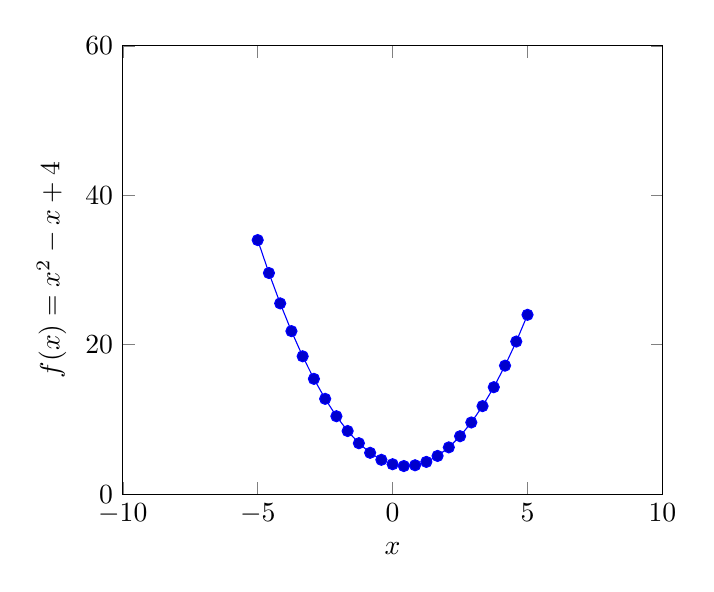
\begin{tikzpicture}
\begin{axis}[
    xlabel=$x$,
    xmin=-10,
    xmax=10,
    ymin=0,
    ymax=60,
    ylabel={$f(x) = x^2 - x +4$},
]
\addplot {x^2 - x +4};
\end{axis}
\end{tikzpicture}
\end{verbatim}
This will get rendered as:
\begin{center}
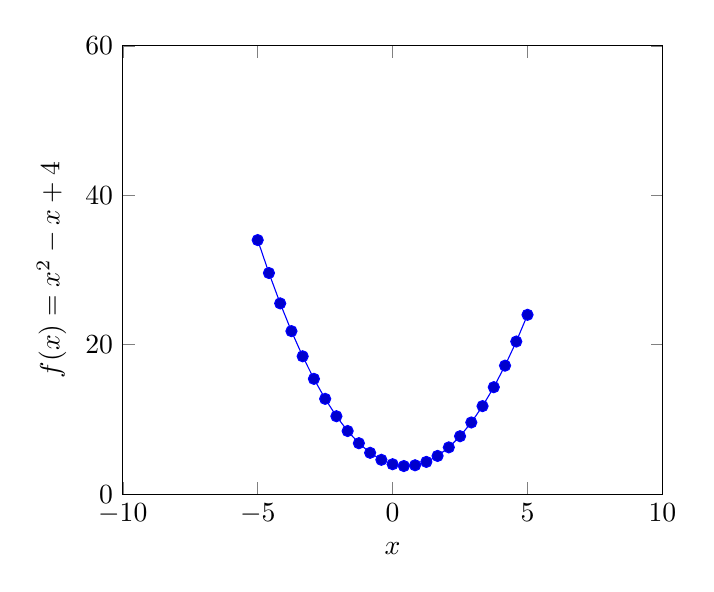
\begin{tikzpicture}
\begin{axis}[
    xlabel=$x$,
    xmin=-10,
    xmax=10,
    ymin=0,
    ymax=60,
    ylabel={$f(x) = x^2 - x +4$}
]
\addplot {x^2 - x +4};
\end{axis}
\end{tikzpicture}
\end{center}
Some other examples of "tikpicture" environment include:\\\\\\
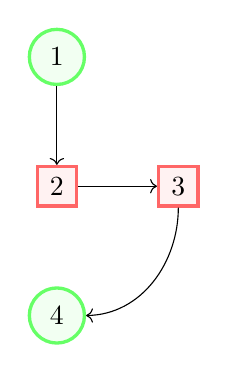
\begin{tikzpicture}[
    roundnode/.style={circle, draw=green!60, fill=green!5, very thick, minimum size=7mm},
    squarednode/.style={rectangle, draw=red!60, fill=red!5, very thick, minimum size=5mm},
]
\node[squarednode]      (maintopic)                              {2};
\node[roundnode]        (uppercircle)       [above=of maintopic] {1};
\node[squarednode]      (rightsquare)       [right=of maintopic] {3};
\node[roundnode]        (lowercircle)       [below=of maintopic] {4};
\draw[->] (uppercircle.south) -- (maintopic.north);
\draw[->] (maintopic.east) -- (rightsquare.west);
\draw[->] (rightsquare.south) .. controls +(down:7mm) and +(right:7mm) .. (lowercircle.east);
\end{tikzpicture}\\\\\\\\

\begin{tikzpicture}
\draw[blue, very thick] (0,0) rectangle (3,2);
\draw[orange, ultra thick] (4,0) -- (6,0) -- (5.7,2) -- cycle;
\end{tikzpicture}\\\\\\\\
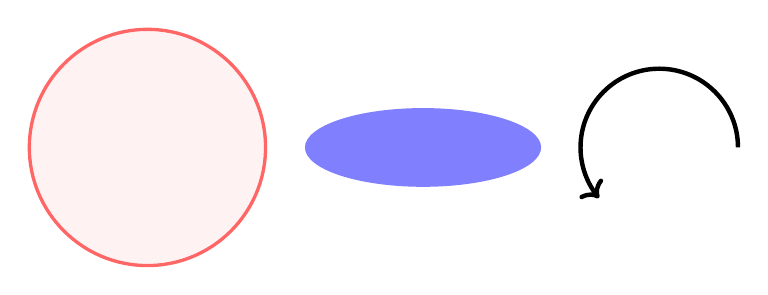
\begin{tikzpicture}
\filldraw[color=red!60, fill=red!5, very thick](-1,0) circle (1.5);
\fill[blue!50] (2.5,0) ellipse (1.5 and 0.5);
\draw[ultra thick, ->] (6.5,0) arc (0:220:1);
\end{tikzpicture}\\\\\\\\
\begin{tikzpicture}
\draw (-2,0) -- (2,0);
\filldraw [gray] (0,0) circle (2pt);
\draw (-2,-2) .. controls (0,0) .. (2,-2);
\draw (-2,2) .. controls (-1,0) and (1,0) .. (2,2);
\end{tikzpicture}\\\\\\\\
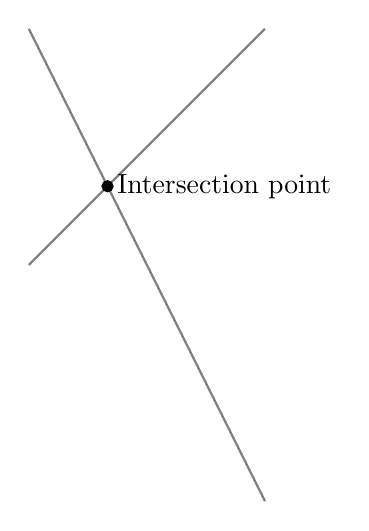
\begin{tikzpicture}
\draw[gray, thick] (-1,2) -- (2,-4);
\draw[gray, thick] (-1,-1) -- (2,2);
\filldraw[black] (0,0) circle (2pt) node[anchor=west] {Intersection point};
\end{tikzpicture}\\\\\\\\
If user adds "circuitikz" package it is possible to create circuit diagrams:\\\\
\begin{circuitikz}
    \draw (0,0)
    to[V,v=$U_q$] (0,2) % The voltage source
    to[short] (2,2)
    to[R=$R_1$] (2,0) % The resistor
    to[short] (0,0);
    \draw (2,2)
    to[short] (4,2)
    to[L=$L_1$] (4,0)
    to[short] (2,0);
    \draw (4,2)
    to[short] (6,2)
    to[C=$C_1$] (6,0)
    to[short] (4,0);
 \end{circuitikz}
\section{Hyperlinks}
To embed clickable links in \LaTeX document import "hyperref" package and use one of following
commands:
\begin{verbatim}
My github page page:\href{https://github.com/mtracewicz}{github.com}\\
My github page page:\url{https://github.com/mtracewicz}\\
\end{verbatim}
Which will get rendered as:\\
My github page page:\href{https://github.com/mtracewicz}{github.com}\\
My github page page:\url{https://github.com/mtracewicz}\\
\end{document}